\section{Introduction}\label{sec:intro}

A coding agent keeps using the wrong naming convention in a repository. An engineer adds one line to its instructions, and the next session follows the convention. The model has not changed, but the deployed system has, as it does when an assistant corrects a stored preference, acquires a reusable skill, or learns which tool to call. We call this persistent layer the \textbf{scaffold}: instructions, skills, memory, tools, orchestration, and the evaluation and governance rules that control their use. In the language of compound AI systems \citep{zaharia2024compound}, it is the part around the model that a deployment can inspect and revise without retraining. Much of the experience that makes a system useful in one setting now accumulates there, and systems that edit it are often described as self-improving.

That label can cover three different things. The first is an artifact that persists: a rule, a memory, or a skill that later sessions load. The second is an edit shown to improve the deployment that made it, which requires running the system again and comparing. The third is an improvement justified somewhere else, which requires evidence from the deployment that receives the edit rather than the one that wrote it. A rule added after one incident may prevent a recurring error, conflict with another rule, or merely lengthen the prompt; a corrected memory may remain in the history while the system goes on retrieving the outdated entry; a rule that helps one repository may be wrong in the next. Persistence settles none of this.

We separate the three as two decisions. The \textbf{local loop} keeps an edit only when a check shows that the deployment's failure rate falls. The \textbf{promotion loop} decides how far a kept edit may travel, to another project, team, or organization, with enough history to reverse that decision. We read 256 public research and production systems by who or what makes each decision: a program, a person, or nothing. The unit of analysis is the decision that accepts a persistent change, not the change.

The two loops are built unevenly. Nearly every system that adapts from failures decides local acceptance by program, while the steps that should feed that check, a log of failures and the trace from a failure to the artifact that caused it, are weaker. Promotion exists only in parts and only inside one operator: no surveyed system connects an automatic local gate to promotion across organizations with versioned lineage, access control, and rollback. The feedback a deployment receives, whether an exact check, an observed outcome, a judgment, or a reward that arrives months later, helps explain this pattern, because it fixes what an acceptance gate can know, and in every class an accepted edit is evidence only for the measure and the tasks it was tested on.

The central contribution is this distinction between keeping, testing, and sharing an edit, and what it reveals about language agents that retain experience, test changes, and transfer learned artifacts. Read through it, the corpus shows four confusions that the self-improvement label can hide: detection mistaken for testing, history mistaken for correction, local success mistaken for transfer, and an evaluator that becomes part of what it evaluates. Around that distinction sit three supporting pieces: a classification of the corpus by who keeps an edit and who lets it travel, a four-class account of what feedback lets a gate know, and an audit of the four properties that governed sharing across organizations would require. The survey runs no experiments. Its classifications are one rater's reading of public evidence, released row by row in the supplementary material so that each can be checked.

\section{Two decisions about an edit}\label{sec:loop}

Learning whether the naming rule works requires running the agent again on relevant tasks and comparing; the local loop makes that comparison routine (Fig.~\ref{fig:loop}). It starts from a record of failures: rejected answers, user corrections, failed tool calls, evaluation regressions, unsuccessful tasks. Repeated failures are grouped into modes and prioritized by frequency and severity. For a selected mode, the system looks for the artifact responsible, since a stale memory entry calls for a different fix from a missing tool argument or an ambiguous instruction. Linking a failure to an editable part of the scaffold, a \textbf{coordinate}, is \textbf{credit assignment}. The system then proposes a candidate edit and tests it against the current scaffold. That test is the \textbf{gate}. An accepted edit is kept as a versioned artifact, and later evidence of regression can trigger rollback.

\begin{figure*}[t]
\centering
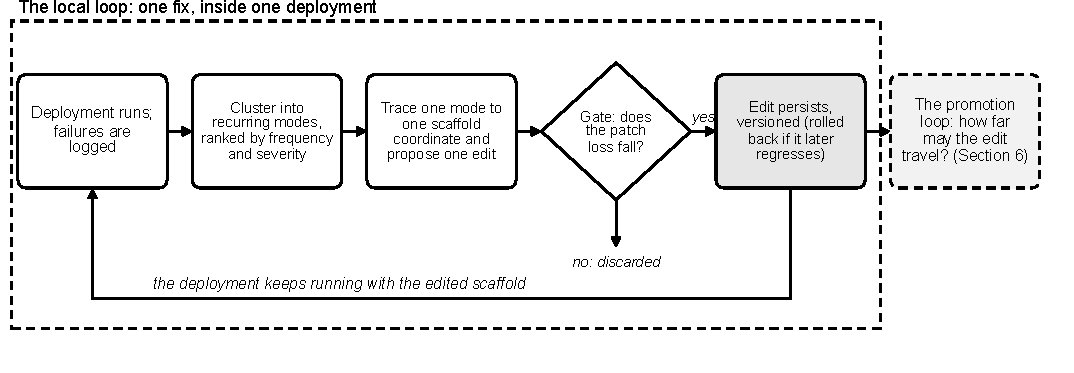
\includegraphics[width=0.92\textwidth]{figures/fig1_descent}
\caption{The local loop. Recurring failures guide a proposed scaffold edit; the local gate tests the change before it persists, and later regressions can trigger rollback. Sharing the kept edit is a separate decision, made by the promotion loop (Section~\ref{sec:promotion}).}
\label{fig:loop}
\end{figure*}

A deployment serves a particular distribution of users, tasks, and conventions, which we call its \textbf{patch}, and its \textbf{patch loss} measures failure on that distribution: a task-failure rate, a correction rate, a retrieval error. Write \(L_D(\theta_s)\) for the patch loss of deployment \(D\) under scaffold \(\theta_s\), with the model weights fixed. No gradient runs through an instruction file, so the gate instead estimates the change in loss that a candidate edit \(z_t\) would cause and accepts the edit only when that estimate clears a margin: \[G_t(z_t)=1\iff\widehat{\Delta}_{z_t}L_D(\theta_s^t)+\lambda\Omega(z_t)\leq-\tau_t,\] where \(\Omega\geq0\) penalizes edit complexity and promotion breadth and \(\tau_t\geq0\) is the acceptance margin. Under further assumptions (Appendix~\ref{app:formal}), improving edits eventually stop clearing the gate. This is \textbf{gate stability}, not global optimality: a limited proposer or a biased evaluator can leave useful changes undiscovered or rejected.

We call maintenance \textbf{artifact-layer descent} when five conditions hold: a measurable patch loss; a failure log that retains relevant failures; credit assignment that, at least sometimes, traces failures to the coordinates responsible; a candidate edit to those coordinates; and an acceptance gate that keeps or promotes an edit only after checking whether it lowers the loss. They separate it from patchwork, where an engineer adds a rule after an incident and measures nothing, and from random artifact search, which tests many variants and keeps a winner without tracing failures to their causes; descent uses the trace to direct the edit and tests the edit before keeping it. Where only some conditions hold, the optimization reading is limited accordingly.

The author of an edit and the authority that accepts it are separate: an agent may draft a revision that a person approves, and an engineer may write one that an automatic evaluation rejects. We classify each gate by who decides. \textbf{Auto} means a program applies a check, such as a verifier, an evaluation threshold, or a language-model judge \citep{zheng2023judge}. \textbf{Human} means a person decides. \textbf{None} means no decision is made, because the loop is absent or every proposed edit is kept. A pair such as {[}Auto \(\times\) Human{]} denotes a program at the local gate and a person at the promotion gate. The labels describe the decision mechanism; they do not by themselves establish that the decision is well supported.

Suppose the naming rule improves its repository and the team considers adding it to a shared template. That decision changes the population the rule acts on: other repositories may follow a different convention, and the local test says little about them. The promotion loop therefore asks for \textbf{receiving-side evaluation}, a check on the tasks of the deployment that would adopt the edit. The \textbf{evidence radius} is the scope for which the available evaluation supports a change, and a local success does not enlarge it. Scopes nest from one person's account (USER) through a repository (PROJECT), a team's bundle of projects (STACK), and an organization (TENANT) to the scope all tenants share (CORE), as drawn in Fig.~\ref{fig:scope} in Appendix~\ref{app:corpus}.

The loss definition puts two limits on every such loop. An accepted edit is evidence of improvement only on the measure and the tasks evaluated, so promotion must preserve that meaning or establish the improvement again. And the loop optimizes a defined objective; it does not discover a better one by accumulating edits. Revising the evaluator changes the objective itself (Section~\ref{sec:evaluator}).

\section{Corpus and reading}\label{sec:method}

We read each system's public method or documentation for four things: the persistent artifact it changes, the feedback that prompts the change, the decision that accepts it, and the scope in which the result is used. The corpus holds 256 systems from January 2023 to an October 2026 cutoff. A system enters if it adapts a foundation model through a persistent artifact updated from deployment signal, or if it is publicly described as self-improving, scaffolded, or agentic; the second group is a contrast set that tests whether those descriptions correspond to persistent adaptation.

Each system is scored from 0 to 5 on six substrates: instructions, skills, memory, tools, orchestration, and governance. A system that scores at least 3 on some substrate joins the core corpus of 204 systems; the other 52 form the contrast corpus. A second filter, the two-loop audit, asks whether session feedback changes a persistent artifact and whether that artifact is then promoted beyond the deployment that produced it, with versioning or lineage.

The audit admits 11 research systems (NanoResearch, SkillOpt, AlphaEvolve, ADAS, DGM, Voyager, SAGE, EvolveR, CoEvoSkills, AutoManual, and CASCADE) and 3 industry exemplars (Sierra Agent OS 2.0, Cognition Devin, and Letta's Context Repositories). Passing does not mean governed sharing. Every passer promotes within one operator, into a shared bank or archive or across the agents and sessions of one deployment, and Letta passes on the lineage of its shared-memory updates although they have no acceptance gate.

A single rater scored every system, rounding ambiguous cases down. Each row of the released table carries its source and a one-line justification. For the 126 most recently added systems, the evidence tier, gate types, feedback class, and governance properties are explicit columns as well, so counts over those columns apply to those systems only (Appendix~\ref{app:corpus}).

\section{What the local loop closes}\label{sec:local}

A system can detect a failure, explain it, and write a plausible fix without ever showing that the fix helps. SkillForge's judge agrees with people more than nine times in ten and picks the replies that should be rewritten. Those replies drive updates to the skill, and nothing tests the rewrite before it is committed \citep{skillforge2026}; the calibration concerns which replies are inadequate, not the effect of the resulting skill change. SkillRL separates the same steps by another route: a success-rate threshold triggers proposals for new skills, and the skill bank accepts each one unconditionally \citep{skillrl2026}. Both systems respond to experience, and both sit in {[}None \(\times\) None{]}. Detection is not testing, which is why the survey records who accepts an edit separately from who writes it or which signal triggers it.

Where a gate exists, it is the best-built step. Of the 126 systems added most recently, 105 are core, and 89 of those keep or reject edits by program. Acceptance also increasingly rests on a body of evidence rather than one favorable run, as in the paired per-item comparisons of SAGE-gate, a statistical acceptance method unrelated to SAGE \citep{wang2026sagegate}, and VaG's three heterogeneous critics that must all pass \citep{shang2026vag}. Averaging independent noisy scores shrinks the variance of their mean, while requiring agreement among independent checks multiplies their false-acceptance probabilities, an idealized gain that real critics, which need not be independent, may not deliver (Appendix~\ref{app:gates}).

The failure log that should feed the gate is rarer. Production memory more often records preferences, successes, or conversation history than failures, and only one field report in the corpus, from a single self-reported deployment, describes a store of dead ends kept to prevent their recurrence \citep{helwig2026memory}. Where failures are retained, nearly every system uses them in arrival order; Task-CoEvolve's variance-weighted task sampling and AutoSaddler's mini-batch failure signals are exceptions \citep{miyai2026taskcoevolve, park2026autosaddler}.

Attribution is harder still. A failed output does not reveal whether its cause was an instruction, a retrieved memory, a skill, or the route through a group of agents; harness-optimization papers repeatedly name this the bottleneck \citep{lin2026ahe, lee2026metaharness}, and by downstream score alone an optimizer cannot be told from trial and error \citep{ong2026harnesseval}. Existing remedies, such as SkillsVote's attribution of an outcome to the skill, the exploration, or the environment before admitting an update \citep{liu2026skillsvote}, usually work inside one substrate. None solves attribution across all six (Appendix~\ref{app:lines}).

Who writes the candidate shapes the loop as much. Research systems usually generate it by reflecting on trajectories; in production prompt platforms an engineer writes it and session feedback never triggers one; and in five public skill repositories every substantive edit was committed under a named human account and merged by a person, most with an AI co-author trailer \citep{shen2026whomaintains}. Instruction files, the most widely deployed artifact (Appendix~\ref{app:corpus}), show what an unmeasured loop leaves open: one controlled study reports higher inference cost without improved task success \citep{gloaguen2026agentsmd}, and another reports lower median wall-clock time and fewer median output tokens, with total tokens about unchanged, without measuring correctness \citep{lulla2026empirical}.

Maintenance also has to remove what no longer helps. Ratchet reports no gain from model-written skills over a no-skill baseline until lifecycle hygiene is applied \citep{zhang2026ratchet}, and eleven surveyed skill systems now treat removal as an operation that must pass a check \citep{zhang2026librarydrift, wei2026skillsmith, pu2026skillops, wang2026assay}.

History is not correction either. Memory products have built one part of maintenance well, recording each entry's history: Letta's Context Repositories use git, Mem0 keeps per-memory history, and Zep represents facts bitemporally \citep{letta2026memfs, mem02026history, zep2026facts}. Yet a study of five production backends finds that all five still return facts that were revoked \citep{shen2026revoked}. The record holds the change, but retrieval does not reliably enforce it.

Correction and reversal have their own limits. A governed collaborative memory that combines provenance, versioning, and correction earns the top memory score in the corpus \citep{cuadros2026governed}. SkillSmith and SkillAudit support edit-level rollback \citep{wei2026skillsmith, gao2026skillaudit}, but VaG finds that reverting a contaminated skill recovers little once other skills have been derived from it \citep{shang2026vag}. The consequences of an edit can outlast the edit.

SkillOpt is a complete instance of all five conditions \citep{yang2026skillopt}. A frozen agent uses one markdown skill document; rollout and reflection batches supply the failure evidence, a consensus filter attributes recurring errors, bounded add, delete, and replace operations propose edits, and a candidate is kept only when its held-out exact-match score strictly improves. The follow-up SkillOpt-Lite drops a rejected-edit buffer and a slow update schedule, keeps the held-out gate and the consensus filter, and matches or exceeds the original \citep{shen2026skilloptlite}; in that setting, the gate and this form of credit assignment carry the weight (Appendix~\ref{app:formal}).

\section{What feedback lets a gate know}\label{sec:signal}

A coding agent changes a repository rule and receives a test result within seconds. A scheduling assistant changes its booking procedure and learns later whether an appointment was made. A marketing assistant changes its tone instructions and receives a reviewer's preference. A research assistant changes its strategy and may wait months to learn whether the direction was productive. All four can propose a persistent edit; what differs is the evidence available for accepting it. The signal's timing, exactness, and dependence on judgment determine how well a gate can estimate the change in loss, and Table~\ref{tab:classes} sorts the corpus into four classes on that basis, each assigned by the constraint that binds first (Appendix~\ref{app:gates}).

\begin{table*}[t]
\centering
\small
\begin{tabular}{>{\raggedright\arraybackslash}p{0.10\textwidth}>{\raggedright\arraybackslash}p{0.21\textwidth}>{\raggedright\arraybackslash}p{0.16\textwidth}>{\raggedright\arraybackslash}p{0.26\textwidth}>{\raggedright\arraybackslash}p{0.12\textwidth}}
\toprule
Class & The signal the gate receives & What the gate can be & What stays hard & Corpus examples \\
\midrule
C1 exact & A check that returns pass or fail, or an exact score, at once and repeatably: tests, compilers, answer keys & An automatic check; one run per case, repeated only to sample the task mix & The lift is bounded and specific, an improvement in what the check measures on the cases it ran; the check names the failed output, not the coordinate that caused it; a check that is also the target can be gamed & DGM, AlphaEvolve, SkillOpt \\
C2 observable outcome & A real result one episode later: a booked slot, a merged pull request, a closed ticket; noisy and confounded & An automatic threshold over batched episodes; a person at promotion & The outcome says \emph{that} the episode failed, not \emph{why}; the channel can be poisoned & Devin, Sierra, SAGE, SkillRL, PACE, Voyager \\
C3 judged & A rater, a rubric, or a model judge; no ground truth & A judge calibrated against people; a person at promotion & The rubric is itself a scaffold coordinate, so the gate judges edits to itself; the proxy gets optimized past the point where it tracks quality & SkillForge, CASCADE, skills-repository review \\
C4 delayed & An outcome weeks or months later, once per many edits & No per-edit gate; proposals are pruned and milestones stand in & Credit across many edits; drift; the loop cannot be told from random search & NanoResearch, CORAL, the AI Scientist \\
\bottomrule
\end{tabular}
\caption{The four feedback-signal classes. Reading across a row: what the gate receives, what it can therefore be, and what it cannot fix.}
\label{tab:classes}
\end{table*}

Exact checks make an automatic gate easy to build, and they also show how narrow its acceptance can be. DGM keeps a self-modification when it passes a sandboxed compile-and-edit functionality check on ten benchmark tasks; the broader benchmark score weights which parent is selected from the archive and does not decide retention \citep{zhang2025darwin}. Exactness belongs to the check, not to the deployment: an agent's outputs are stochastic, a finite suite samples only part of the task distribution, and passing the suite establishes only the properties it tests.

Observed outcomes are meaningful but noisy and confounded. A user can accept a wrong answer, and a merged pull request reflects more than the agent's technical work; Devin nonetheless reads merged pull requests as feedback \citep{cognition2025devinreview}. Simulated outcomes, as in Voyager's game world or SAGE's AppWorld \citep{wang2025sage}, remove the user confound and can be sampled again. In both cases an automatic gate needs a positive margin and enough episodes to absorb noise, and the result reveals that a task failed more readily than why.

Judged feedback has no independent answer to check against. For style, persuasion, design, and other preference-dependent tasks, the gate is a person, a rubric, or a model judge, and a judge's score counts as evidence of the preference only after it is calibrated against the people it stands in for. An uncalibrated judge is still an Auto gate, though its acceptances mean less. SkillForge, SkillChain, and SkillCoach report calibration measurements \citep{skillforge2026, hu2026skillchain, zhu2026skillcoach}; no other surveyed judge does.

Delayed outcomes remove per-edit acceptance altogether. When a research direction is judged months later, after many intervening edits, the outcome cannot be assigned to each scaffold change. NanoResearch merges skills by semantic compatibility \citep{xu2026nanoresearch} and CORAL promotes findings into shared memory on a heartbeat \citep{qu2026coral}; these prune or consolidate proposals without estimating any edit's contribution to the eventual loss.

The classes yield three expectations. Local automatic acceptance should rest most directly on exact checks and observed outcomes; automatic promotion that estimates a loss change should appear only where a comparable check can run at the recipient, with people holding promotion for observed outcomes and judgments; and the dominant risks should differ by class, from suite overfitting and bloat under exact checks to drift under delay. The gate grid in Section~\ref{sec:promotion} bears out the first two once one qualification is explicit: a program can merge two judged artifacts or prune a delayed proposal without estimating a loss change, so these are expectations about what a gate can establish, not about what software can execute. The failure surface in Appendix~\ref{app:failure} sorts by class as the third expects, although no risk belongs to one class alone. In every class, an accepted edit is evidence only for the measure and the tasks it was tested on.

\section{When an improvement is shared}\label{sec:promotion}

Copying a rule file transfers the instruction, not the evidence that justified it. The recipient must either share the relevant evaluation conditions or test the change on its own workload, and a lower average loss at a broad scope can hide harm to one recipient. Local success is not transfer. A few systems already gather evidence beyond the source deployment, inside one operator. ShareMem consolidates one user's memories for another and evaluates them in the receiving context \citep{hu2026sharemem}; XRepoSkill verifies a rule in at least two repositories \citep{guo2026xreposkill}; Evo2Team promotes routing skills between teams and confirms them at the target \citep{wang2026evo2team}. Confirmation is necessary, not sufficient. Even in Evo2Team, nearly a fifth of confirmed transfers fail on graphs the confirmation did not cover.

Federated systems place the check elsewhere. EvolveNet merges a shared harness only when the merge fixes at least as many held-out items as it breaks, but the check runs at the aggregator \citep{nie2026evolvenet}; FederatedSkill's server agent applies, adapts, or rejects each client's edit \citep{yang2026federatedskill}. Their clients are partitions or agent instances under one operator, not independently governed organizations, so neither instantiates a gate at a receiving organization.

Who lets an edit climb divides the corpus three ways. Research systems often promote by program, admitting a candidate to a bank or archive that later runs reuse; SkillOpt, DGM, ADAS, Voyager, SAGE, and AlphaEvolve decide this way \citep{hu2024adas, wang2023voyager, alphaevolve2025}. That pool, inside one operator, is as far as any of them travels, with no access control, audited promotion, or gate at a receiving organization. Automatic admission also varies in what it means: NanoResearch's semantic merge, AutoManual's judged rewriting and consolidation, and ShareMem's judged consolidation are programmatic decisions, but none estimates a candidate's reduction in patch loss.

Production systems more often keep a person at the promotion gate. Sierra routes generated insights through human-authored expert answers \citep{sierra2025os20}; in Devin, one pull-request merge both supplies the local outcome and records the reviewer's approval; and the research system CASCADE also combines human and agent approval for memory consolidation \citep{huang2025cascade}. The person stands in for the exact signal production lacks, which makes a program at the local gate and a person at the promotion gate the production-viable pairing rather than a compromise. Letta takes a third path, pushing shared-memory changes with git lineage and no acceptance check, while AutoAgent propagates nothing \citep{wang2026autoagent}. Both receive None at the promotion gate, one for sharing without checking and the other for not sharing.

Much of the sharing infrastructure exists apart from any learning loop. Coding assistants have converged on git-tracked markdown artifacts, with a tool layer organized around MCP-style interfaces \citep{galster2026harnessconfig}, yet the runtime state of the adaptation process stays outside version control \citep{lulla2026loopengineering}. MCP registries add namespaces and version records, governance registries add lineage and rollback, and prompt platforms such as Braintrust and LangSmith Hub add immutable versions, evaluation thresholds, and rollback \citep{braintrust2026docs, langsmith2026hub}. Engineers author the candidates, and none of these systems generates one from failures. They move artifacts without carrying evidence that an artifact helps its recipient.

\begin{figure}[t]
\centering
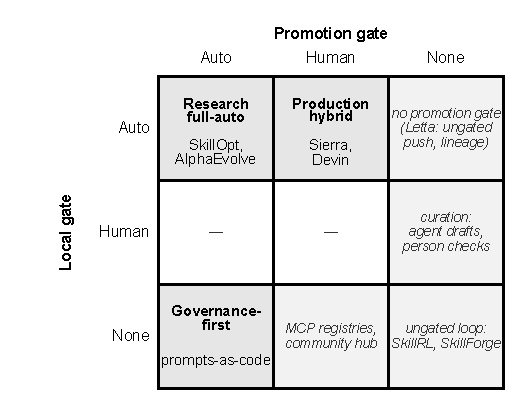
\includegraphics[width=\columnwidth]{figures/fig3_design_space}
\caption{Local and promotion gates. Each axis records who accepts a change: a program (Auto), a person (Human), or no gate (None). None at the promotion gate includes both absent promotion and unchecked sharing; Section~\ref{sec:promotion} distinguishes these cases, and Appendix~\ref{app:grid} lists the occupants of each cell.}
\label{fig:grid}
\end{figure}

Fig.~\ref{fig:grid} places the two gates on one grid. {[}Auto \(\times\) Auto{]} holds research systems that close both loops inside one environment or one operator; where their promotion gate estimates a loss change, the signal is an exact check or a simulated outcome. {[}Auto \(\times\) Human{]} holds production systems with a reviewer on promotion, and CASCADE, with no exact-signal system. {[}Human \(\times\) Auto{]} and {[}Human \(\times\) Human{]} are empty: human local decisions occur only in curation, such as SkillChain's reflection gate, where a person decides which refined skills are deployed \citep{hu2026skillchain}, and curation promotes nothing. The bottom row holds prompt platforms, registries, and community hubs with no failure-driven loop, and {[}None \(\times\) None{]} holds SkillRL and SkillForge. No relaxation of the audit yields governed promotion across organizations (Appendix~\ref{app:grid}). No system has both the learning of the top row and the governance of the bottom.

\section{When the evaluator changes}\label{sec:evaluator}

A pitch-review assistant consistently overrates decks that claim a large market without supporting numbers. The team revises its rubric from ``evaluate market size'' to ``require a numeric estimate and a source.'' The edit may improve reviews, but it also changes the standard that will judge later behavior. If the same rubric judges future rubric revisions, the improvement process is modifying its own measuring instrument: the rubric is itself a scaffold coordinate, so the gate judges edits to itself. We call this the \textbf{reflexive gate}.

Calibration is the obvious defense, and it is missing exactly here: of the three scaffold systems that report calibrating a judge against people, none reports it for a judge that is itself being edited. The gap is keeping calibration while the criterion moves, which means evaluating the moving criterion as well as the outputs it scores. A fixed evaluator is not safe either. Optimizing a proxy beyond a point reduces the quality it was meant to track \citep{gao2023overoptimization}, and human evaluators' criteria change as they grade more outputs \citep{shankar2024validators}. A gate needs its own held-out checks, calibration where judgment is involved, and a revision history.

Weight-level reinforcement learning meets the same problem when it extends verifiable rewards to open-ended tasks: some methods hold the judge fixed \citep{gunjal2025rubrics}, others update the reward, rubric, or judge alongside the policy \citep{xu2026rubricarm, ding2026evorubrics}, and among the co-evolving methods reviewed only RLPR reports agreement with human labels, with a reward that is a probability rather than a rubric \citep{yu2025rlpr}. The reflexive gate is one entry on a wider failure surface that includes scaffold bloat, poisoned memory, injection through tools, coordination failures, and drift. The literature, not this corpus, measured six of those failures (Appendix~\ref{app:failure}).

\section{Related work}\label{sec:related}

Neighboring surveys organize the field by what, when, how, and where an agent evolves \citep{gao2026selfevolving}, by inputs, agent system, environment, and optimizer \citep{fang2025comprehensive}, by the authority, scope, mutability, provenance, and recoverability of persistent state \citep{ding2026alwayson}, or by lifecycle phase and security objective for memory \citep{lin2026memorysecurity}. The last two are the closest governance precedents, and neither asks who gates an edit. None of the surveys classifies the gate that accepts an edit, the feedback that supports it, and the scope the edit reaches, and none covers promotion across organizations (Appendix~\ref{app:surveys}).

Prompt optimization supplies a second lineage. OPRO, DSPy, TextGrad, and their relatives optimize a prompt or program once against development evidence \citep{yang2023opro, khattab2023dspy, yuksekgonul2024textgrad}; they are not deployed loops. ACE persists an evolving playbook but never promotes it \citep{ace2025agentic}. These works establish many of the mechanisms read here. What they leave to this survey is the joint reading at deployment scope: whether an artifact persists, whether a local acceptance decision is made, which signal supports it, and what authorizes its use elsewhere.

A third body of work built the loop in pieces. Reflective evolution supplied proposal from trajectory evidence \citep{agrawal2025gepa}; reflective context learning supplied a generalization penalty, the \(\Omega\) of the gate \citep{vassilyev2026rcl}; harness optimization supplied attribution within the orchestration graph \citep{lee2026metaharness, nguyen2026harnessevo}; the lifecycle literature supplied gated retirement; and transfer and federation supplied the check on arrival. Each line inherited its loss from a benchmark and began from available trajectories, and building a record of recurring failures was none of their starting problems. This history helps explain why the local loop grew from evaluation backward toward the evidence needed to choose a useful edit (Appendix~\ref{app:lines}).

\section{Discussion and open problems}\label{sec:discussion}

Why specialization should live outside the weights has a practical answer and a structural hypothesis. A deployment must follow its own conventions and avoid failures that are rare globally but frequent locally; per-customer adapters \citep{hu2021lora} can absorb some of this but bring separate training, evaluation, and serving lifecycles, and in practice they are rare. Adaptation lands in persistent artifacts, the one substrate that is cheap, inspectable, reversible, scoped to one customer, and updatable daily (Appendix~\ref{app:why}).

The structural hypothesis comes from two analyses of error. \citet{arbuzov2025beyond} argue that long-output reliability depends on a sparse set of key decisions rather than a uniform error probability at every token, an argument supported by long-range dependence measured on one natural-text corpus and by majority-voting gains on reasoning benchmarks, and limited when consequential decisions grow with the task, as in long-horizon agentic work. \citet{arbuzov2026architecture} argue that in a bounded deployment with recurring tasks, tools, and evaluator expectations, failures fall into a catalogue of modes that grows slowly with experience, so that under their assumptions the intervention budget grows polylogarithmically with sequence length and becomes constant once the catalogue saturates, while a finite catalogue cannot cover an unbounded domain. If these hypotheses generalize, a deployment may be improved through a manageable set of targeted interventions, persistent artifacts give those interventions an inspectable form, and on that hypothesis the gated, scoped artifact layer is not a workaround for an inadequate model but the architecture the error structure calls for. The survey does not test the hypotheses; its findings about gates, feedback, and promotion follow from the corpus independently of them.

Governed sharing across organizations is a consequence of these findings, not their motivation. It needs four properties at once: an auto-gated local loop, promotion between independently governed organizations, versioned lineage with access control, and rollback. FederatedSkill and EvolveNet come closest and stay within one operator. No surveyed system holds all four, and none rolls back a promotion across organizations, because none makes one. Where quality is judged, a human promotion gate is a design feature (Appendix~\ref{app:governed}).

The open problems follow the decisions: attributing a failure to its editable cause across artifact types, where slot, intervention-based, and contrastive attribution offer narrower starting points \citep{nguyen2026harnessevo, chu2026agentgrad, zehle2026cantante}; evaluation at the receiving deployment, which Federated Agent Optimization proposes but does not implement \citep{yang2026fao}; keeping a judge calibrated while its rubric is edited; and evaluation under delayed reward, where an optimizer should be held to its claims about why an edit helps and not only to its final score. Only after those can governed sharing across organizations join the parts while preserving tenant isolation and accounting for artifacts derived from a change that is later withdrawn.

The frontier model generalizes. The local scaffold specializes. Reliability comes from governing that specialization: knowing what each change improved, where that evidence applies, and how the change can be reversed, including when the change is to the evaluator itself.
